%%%%%%%%%%%%%%%%%%%%%%%%%%%%%%%%%%%%%%%%%%%%%%%%%%%%%%%%%%%%%%%%%
%%% %
%%% % weiiszablon.tex
%%% % The Faculty of Electrical and Computer Engineering
%%% % Rzeszow University Of Technology diploma thesis Template
%%% % Szablon pracy dyplomowej Wydziału Elektrotechniki 
%%% % i Informatyki PRz
%%% % June, 2015
%%%%%%%%%%%%%%%%%%%%%%%%%%%%%%%%%%%%%%%%%%%%%%%%%%%%%%%%%%%%%%%%%

\documentclass[12pt,twoside]{article}

\usepackage{weiiszablon}
\usepackage{fancyhdr}
\usepackage{amsmath}
\usepackage{graphicx}
\usepackage{graphicx}
\usepackage{subcaption}
\usepackage{verbatim}

\fancyhf{} % Wyczyść bieżące ustawienia stopki
% Ustawienia dla lewego rogu stopki
\fancyfoot[L]{D.K.}

% Ustawienia dla prawego rogu stopki
\fancyfoot[R]{\thepage}


\author{Daniel Kleczyński}

% np. EF-123456, EN-654321, ...
\studentID{EF-167802}

\title{Badanie niektórych parametrów konwolucyjnej sieci głębokiej używając zbioru obrazów WHU-RS19 }
\titleEN{Temat pracy po angielsku}


%%% wybierz rodzaj pracy wpisując jeden z poniższych numerów: ...
% 1 = inżynierska	% BSc
% 2 = magisterska	% MSc
% 3 = doktorska		% PhD
%%% na miejsce zera w linijce poniżej
\newcommand{\rodzajPracyNo}{0}


%%% promotor
\supervisor{dr hab. inż. Roman Zajdel, prof. PRz}
%% przykład: dr hab. inż. Józef Nowak, prof. PRz

%%% promotor ze stopniami naukowymi po angielsku
\supervisorEN{(academic degree) Imię i nazwisko opiekuna}

\abstract{Treść streszczenia po polsku}
\abstractEN{Treść streszczenia po angielsku}

\fancyhf{} % Wyczyść bieżące ustawienia stopki
% Ustawienia dla lewego rogu stopki
\fancyfoot[L]{D.K.}

% Ustawienia dla prawego rogu stopki
\fancyfoot[R]{\thepage}

\begin{document}




\author{L8 2EF-DI \\ Daniel Kleczyński}

% strona tytułowa
\maketitle



% spis treści
\tableofcontents

\clearpage



\section*{Wprowadzanie}
\addcontentsline{toc}{section}{Wprowadzanie}%
Głębokie sieci konwolucyjne (ang. deep convolutional neural networks, CNN) są rodzajem modeli głębokiego uczenia maszynowego, które są szczególnie skuteczne w analizie i przetwarzaniu danych wizyjnych, takich jak obrazy i filmy. Ich zastosowanie obejmuje wiele dziedzin, takich jak rozpoznawanie obrazów, segmentacja, detekcja obiektów, klasyfikacja i wiele innych.

Sieci konwolucyjne składają się z  kilku warstw konwolucyjnych, które ekstrahują cechy z danych wejściowych poprzez przeprowadzenie operacji konwolucji na obrazach. Operacje konwolucji polegają na nakładaniu filtrów na obrazy i obliczaniu ich odpowiedzi. Filtry te uczą się automatycznie w procesie trenowania, aby wyodrębnić istotne wzorce i cechy z obrazów.

Głębokie sieci konwolucyjne składają się z wielu warstw konwolucyjnych, które są stosowane sekwencyjnie. Zazwyczaj zaczynają się od prostych filtrów, które wykrywają podstawowe cechy, takie jak krawędzie i tekstury, a następnie kolejne warstwy wykrywają coraz bardziej skomplikowane wzorce. W miarę postępu w głąb sieci, abstrakcyjność cech rośnie, co pozwala na bardziej zaawansowane rozumienie i interpretację obrazów stosuje się również klasyczne warstwy neuronów które mogą posłużyć do przekształcenia na klasyfikator przykładowy schemat sieci CNN rysunek \ref*{fig:klasyczny_CNN}  .
\begin{figure}[ht]
	\centering
	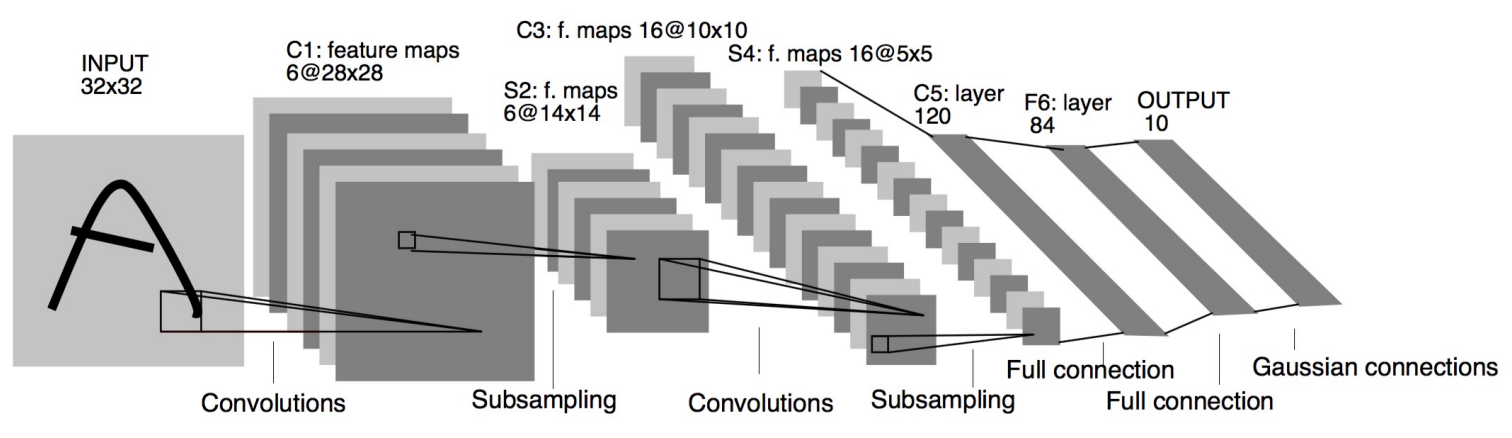
\includegraphics[width=0.9\textwidth]{figures/klasyczyn_CNN.png}
	\caption{Archtektura sieci konwolucyjnych}
	\label{fig:klasyczny_CNN}
  \end{figure}


  Zastosowanie głębokich sieci konwolucyjnych ma szerokie spektrum. W dziedzinie rozpoznawania obrazów, CNN może być wykorzystywany do klasyfikacji obiektów na obrazach, np. rozpoznawanie gatunków zwierząt lub identyfikowanie przedmiotów. Mogą również być stosowane do detekcji obiektów, gdzie sieć może wykrywać obiekty na obrazie i określać ich położenie.

Sieci konwolucyjne są również wykorzystywane w segmentacji obrazu, gdzie mogą dzielić obraz na różne regiony lub piksele należące do różnych klas. Ponadto, CNN znalazły zastosowanie w dziedzinach takich jak rozpoznawanie mówcy, analiza medyczna, przetwarzanie naturalnego języka i wiele innych.






\clearpage

\section{Problemeatyka oraz charakterystyczne rozwiązania w głębokich sieciach CNN w zastosowaniu klasyfikacji zdjęć } 

W celu uczneia algorymów coraz bardzief skąplikowanych zależność wielkość warstw oraz głępokość sieci była stale powiększana w przypadku algorytmów MLP skutkowało to bardzo dużą ilością 
paramertów do ucznia. Rozwązaniem były warstwy konwolucyjne oraz inne rozwązania. 

\subsection{Problematyka zanikającego gradnietu}

Problem zanikającego gradientu występuje, gdy w trakcie propagacji wstecznej gradient maleje wraz z głębokością sieci, co prowadzi do trudności w uczeniu głębokich warstw. Wzór na zanikający gradient można przedstawić w następujący sposób:

Niech $\frac{\partial J}{\partial W}$ oznacza gradient funkcji kosztu $J$ względem wag $W$. Wówczas gradient dla danej warstwy można obliczyć jako iloczyn gradientu warstwy powyżej i pochodnej funkcji aktywacji. Przykładowo, dla dwóch warstw:
$$\delta_2 = \frac{\partial J}{\partial A_2} \cdot g'(z_2)$$
$$\delta_1 = W_2^T \cdot \delta_2 \cdot g'(z_1)$$

gdzie:
\begin{itemize}
	\item $\delta_2$ to gradient dla warstwy drugiej (bliżej wyjścia)
	\item $\delta_1$ to gradient dla warstwy pierwszej (bliżej wejścia)
	\item $\frac{\partial J}{\partial A_2}$ to gradient funkcji kosztu $J$ względem wyjścia warstwy drugiej
	\item $g'(z)$ to pochodna funkcji aktywacji względem wejścia $z$
	\item $z_2$ to wejście do warstwy drugiej
	\item $W_2$ to macierz wag dla warstwy drugiej
	\item $z_1$ to wejście do warstwy pierwszej
\end{itemize}

Problem zanikającego gradientu występuje, gdy pochodna funkcji aktywacji $g'(z)$ jest mała (bliska 0) dla większości wartości $z$ w obszarze, w którym znajduje się większość danych. W takiej sytuacji, iloczyn $W_2^T \cdot \delta_2 \cdot g'(z_1)$ może również stać się bardzo mały, co prowadzi do zanikania gradientu dla warstwy pierwszej. To z kolei powoduje, że wagi w warstwie pierwszej nie są aktualizowane w odpowiedni sposób, co utrudnia efektywne uczenie sieci.

\subsection{Charakterystyczne  rozwiązania w głębokich sieciach CNN }

Aby radzić sobie z problemem zanikającego gradientu, stosuje się różne techniki, takie jak:

\begin{itemize}
	\item Użycie innych funkcji aktywacji, które nie mają tendencji do zanikania gradientu, na przykład funkcji ReLU (Rectified Linear Unit).
	\item Inicjalizacja wag w sposób bardziej odpowiedni, na przykład przy użyciu inicjalizacji Xavier/Glorot.
	\item Normalizacja danych lub warstw w celu zmniejszenia zakresu wartości wejściowych.
	\item Wykorzystanie architektur sieci, które umożliwiają przepływ gradientu na większe odległości, takie jak sieci rekurencyjne (RNN) lub połączenia pomijające (skip connections) w sieciach konwolucyjnych.

\end{itemize}

Dzięki tym technikom można zminimalizować problem zanikającego gradientu i umożliwić skuteczne uczenie głębokich sieci neuronowych.

\subsubsection{Funkcja aktywacji ReLU}

Funkcja ReLU jest popularną funkcją aktywacji w sieciach neuronowych, ponieważ ma prostą i efektywną implementację oraz pomaga w rozwiązaniu problemu zanikającego gradientu. Funkcja zwraca wartość zero dla wszystkich wartości wejściowych mniejszych niż zero, a dla wartości nieujemnych zwraca wartość równą wejściu.


$$
f(x) = \begin{cases}
0, & \text{dla } x < 0, \\
x, & \text{dla } x \geq 0.
\end{cases}
$$

Funkcja ta jest prostą nieliniową funkcją, która działa jako prosta przekształcenie dla wartości nieujemnych i przepuszcza je bez zmian. Jeśli wartość wejściowa jest ujemna, funkcja zwraca 0. 
Graficznie, funkcja ReLU można przedstawić jako prostą linię przechodzącą przez punkt (0,0), a dla wartości ujemnych osiąga wartość 0, a dla wartości nieujemnych zachowuje się jak funkcja tożsamościowa.
Funkcja ReLU jest popularna ze względu na jej prostotę obliczeniową oraz zdolność do rozwiązywania problemu zanikającego gradientu,Ponadto, ReLU jest nieodwracalna, co może wprowadzić do modelu nieliniowość i zdolność do wykrywania i reprezentowania złożonych wzorców i relacji w danych.


\subsubsection{Inicjalizacja wag przy użyciu Xavier/Glorot.}

Xavier (również znane jako inicjalizacja Glorot) to popularna metoda inicjalizacji wag w sieciach neuronowych. Metoda ta ma na celu zapewnienie odpowiedniej skali wag na początku uczenia, aby uniknąć zanikającego gradientu.

Inicjalizacja Xavier/Glorot opiera się na rozkładzie normalnym lub jednostajnym w zależności od funkcji aktywacji. W przypadku rozkładu normalnego, wagi są inicjalizowane zgodnie z następującym wzorem:

\[
W \sim N\left(0, \frac{1}{\sqrt{n_{\text{in}}}}\right)
\]

gdzie:
\begin{itemize}
  \item $W$ to macierz wag,
  \item $N(\mu, \sigma)$ to rozkład normalny o średniej $\mu$ i odchyleniu standardowym $\sigma$,
  \item $n_{\text{in}}$ to liczba neuronów w poprzedniej warstwie.
\end{itemize}

Natomiast w przypadku rozkładu jednostajnego, wagi są inicjalizowane zgodnie z następującym wzorem:

\[
W \sim U\left(-\frac{\sqrt{6}}{\sqrt{n_{\text{in}} + n_{\text{out}}}}, \frac{\sqrt{6}}{\sqrt{n_{\text{in}} + n_{\text{out}}}}\right)
\]

gdzie:
\begin{itemize}
  \item $U(a, b)$ to rozkład jednostajny o przedziale $(a, b)$,
  \item $n_{\text{out}}$ to liczba neuronów w bieżącej warstwie.
\end{itemize}

Inicjalizacja Xavier/Glorot pozwala na równomierne rozprowadzenie wariancji wejść i wyjść neuronów, co sprzyja stabilnemu uczeniu sieci neuronowej. Dzięki temu metoda ta może pomóc w uniknięciu zanikającego lub eksplodującego gradientu na początku uczenia.

\subsubsection{Normalizacja danych lub warstw}
Normalizacja danych lub warstw jest powszechną techniką stosowaną w sieciach neuronowych w celu zmniejszenia zakresu wartości wejściowych. Ma to na celu ułatwienie uczenia się modelu poprzez zapewnienie bardziej stabilnego i efektywnego procesu optymalizacji. Istnieją różne metody normalizacji danych lub warstw, a niektóre z najpopularniejszych to:

\begin{itemize}

\item Normalizacja z-score (standardowa normalizacja)

\item Normalizacja min-max
Ta metoda przekształca wartości danych w zakres od 0 do 1. 

\item Batch Normalization (normalizacja wsadowa)

\item Layer Normalization (normalizacja warstwowa)

\end{itemize}


\subsubsection{ Architektur sieci, które umożliwiają przepływ gradientu w głąb sieci }

Sieci konwolucyjne z połączeniami pomijającymi (skip connections) są rozwinięciem tradycyjnych sieci konwolucyjnych, które mają na celu rozwiązanie problemu zanikającego gradientu oraz wzmocnieniu nisko abstrakcjnych cech obrazu.

W sieciach konwolucyjnych z połączeniami pomijającymi wprowadza się dodatkowe połączenia, które tworzą skoki w przepływie informacji. Te połączenia łączą warstwy wcześniejsze bezpośrednio z warstwami późniejszymi, pomijając niektóre pośrednie warstwy konwolucyjne rysunek \ref{fig:skip_cone}. Dzięki temu połączeniu informacja o niskopoziomowych cechach może być bezpośrednio przenoszona do warstw wyższego poziomu.

\begin{figure}[ht]
	\centering
	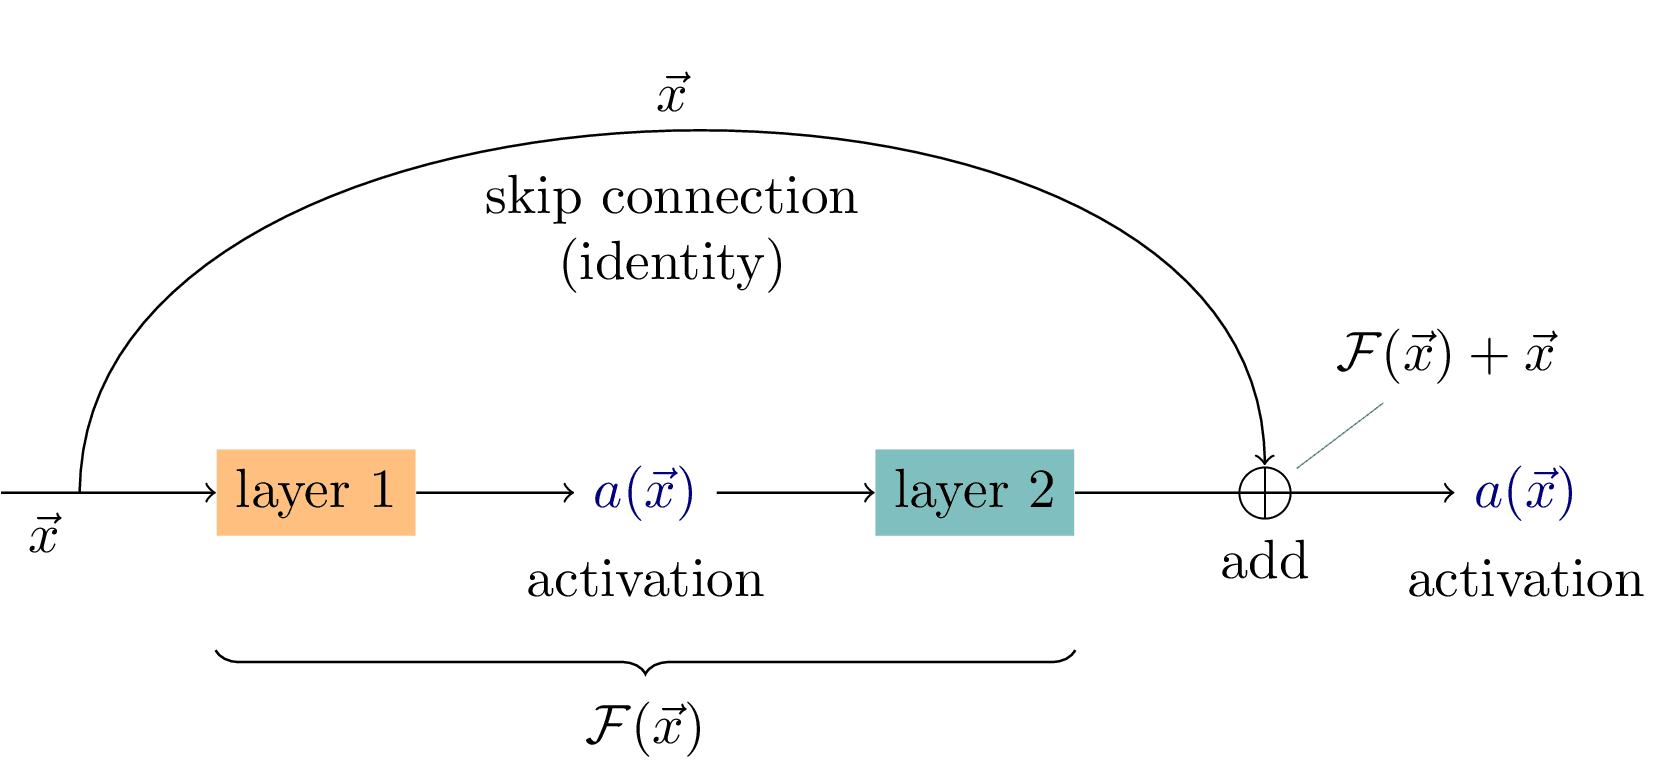
\includegraphics[width=0.9\textwidth]{figures/skip-connection.png}
	\caption{Architektura z połączeniami pomijającymi}
	\label{fig:skip_cone}
  \end{figure}

Główną korzyścią wynikającą z wykorzystania połączeń pomijających jest możliwość przekazywania i zachowywania informacji o niskopoziomowych cechach, które są istotne dla skutecznego uczenia się sieci. Dzięki temu sieć może efektywniej wykorzystać te cechy do dokładniejszej klasyfikacji lub predykcji. Ponadto, połączenia pomijające umożliwiają propagację gradientu wstecznie z wyższych warstw do niższych warstw, co ułatwia proces uczenia się i przeciwdziała zanikaniu gradientu.
\clearpage

\section{Dane uczące oraz ich przygotowanie}




W procesie uczenia będzie używany zbiór WHU-RS19 o liczebnośći 1005 jest to zbiór Kwadratowych kolorowych zdjęć o rozmiach 600x600 px w formacie .jpg. Zrobone Satelitarnie Zdjęcia przedsatiają  obiekty takie jak  'Airport',
'Beach',
'Bridge',
'Commercial',
'Desert',
'Farmland',
'Forest',
'Industrial',
'Meadow',
'Mountain',
'Park',
'Parking',
'Pond',
'Port',
'Residential',
'River',
'Viaduct',
'footballField',
'railwayStation'  ich liczebnoś jest zaprzentowana na wykresie \ref{fig:dane}

\begin{figure}[ht]
	\centering
	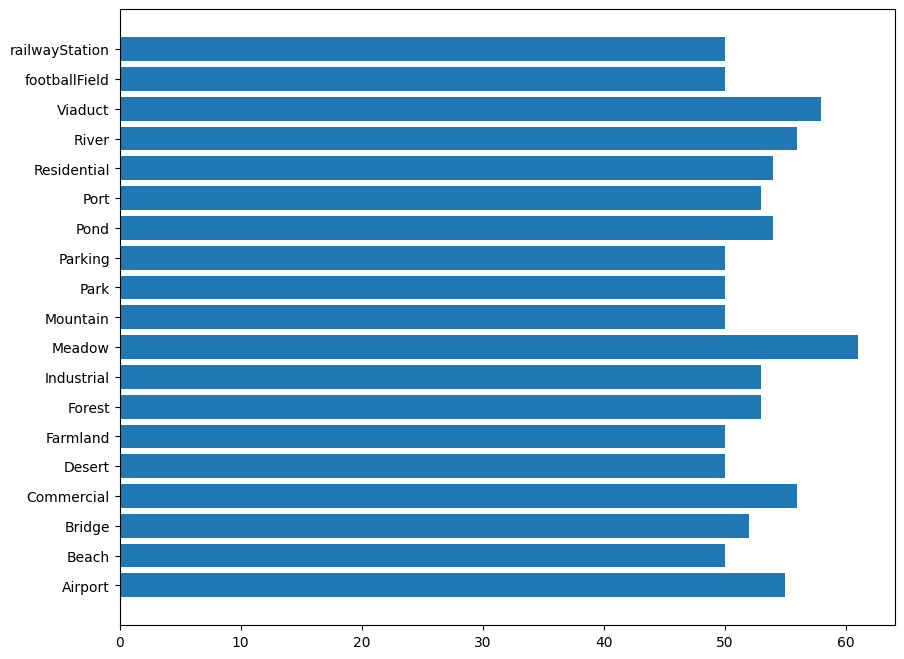
\includegraphics[width=0.9\textwidth]{figures/dane_class.png}
	\caption{Zestawienie liczebnośći zdjęć w poszczególnych klasach}
	\label{fig:dane}
  \end{figure}

Dane w takiej konfiguracj nie są odpowiednie do uczeniea składa się na to kilka cech takich jak zbyt duży rozmiar zdjęcia co powoduje  znaczne zwiększenie danych wejściowych oraz obecny format który nie jest w staenie być przetwarzany na jednostkach obliczniowych 'cuda' a to rówinież wydłuża proces ucznia.
Na zdięciach zostanie przepowadzona transforamcja do typu danych jakim są trnsory o rozmiarach \texttt{tensor(1, 3, 384, 384)} 
Poszczególne wymiary mają następujące znaczenie:
\begin{itemize}
	\item (1): Odpowiada liczbie przykładów w zbiorze danych. W tym przypadku mamy tylko jeden przykład.
	\item (3): Odpowiada liczbie kanałów koloru. W przypadku obrazów w formacie RGB.
	\item  (384): Odpowiada liczbie pikseli w pionie (wysokość obrazu) przedział wartości.
	\item (384): Odpowiada liczbie pikseli w poziomie (szerokość obrazu).

\end{itemize}
odpowiada za to taka transformacja: 

\begin{lstlisting}[language=Python,caption=Transforamcja zdjęć,label={kod_Transformacja}]
	self.transform = transforms.Compose([
            transforms.Resize((384, 384)),
            transforms.ToTensor(),
        ])
\end{lstlisting}

Typ danych przechowywanych w tensorach to \texttt{float32} z sakresu od 0 do 1 (po normalizacji przed użyciem w sieci).


\begin{figure}[b]
	\centering
	\includegraphics[width=0.9\textwidth]{figures/przykłady_zdj.png}
	\caption{Przykłady zdjęć}
	\label{fig:dane}
  \end{figure}

przykład pojedynczego tensora pokazenie tylko wymiarów 2 i 3 : 

  \begin{verbatim}
	tensor([[[0.2510, 0.2196, 0.2157,  ..., 0.2392, 0.2275, 0.2196],
         [0.2980, 0.2667, 0.2549,  ..., 0.2863, 0.2784, 0.2784],
         [0.3294, 0.3098, 0.3059,  ..., 0.3333, 0.3294, 0.3373],
         ...,
         [0.5843, 0.4902, 0.4627,  ..., 0.2980, 0.3059, 0.3176],
         [0.5569, 0.5020, 0.4667,  ..., 0.3020, 0.3020, 0.3137],
         [0.5490, 0.5176, 0.4745,  ..., 0.3098, 0.3059, 0.3059]],...

\end{verbatim}

\clearpage
\section{Przedstwienie oraz omówienie własnej archtektury CNN}

Architektura sieci Lstlisting \ref{MyModel1} jest oparta na rozwiązaniach biblioteki PyTorch posiada ona 197 000 parametrów do nauki, 3 warstwy konwolucyjne , 1 warstwę neuronów ReLU, 1 warstwę neuronów linowych, 2 bloki Sequential gdzie każda z nich składa się z 2 warstw Relu oraz 2 warstw konwolucyjnych

\begin{lstlisting}[language=Python,caption= Struktura głębokiej sieci konwolucyjnej MyModel1 ,label={MyModel1}]
	class MyModel1(nn.Module):
    def __init__(self, num_classes=19):
        super().__init__()
        self.conv1 = nn.Conv2d(3, 64, kernel_size=3, stride=1, padding=1)
        self.relu1 = nn.ReLU()
        self.conv2 = nn.Conv2d(64, 64, kernel_size=3, stride=1, padding=1)
        self.residual1 = self._make_residual_block(64, 64)
        self.residual2 = self._make_residual_block(64, 64)
        self.skip_connection = nn.Conv2d(128, 64, kernel_size=1, stride=1)   
        self.max_pool = nn.MaxPool2d(kernel_size=2)
        self.fc = nn.Linear(64, num_classes)
        self._initialize_weights()
    def forward(self, x):
        out = self.conv1(x)
        out = self.relu1(out)
        out = self.conv2(out)
        residual1 = self.residual1(out)
        residual2 = self.residual2(residual1)
        skip_out = self.skip_connection(torch.cat([residual1, residual2], dim=1))
        skip_out = self.max_pool(skip_out)  
        out = self.max_pool(out) + skip_out
        out = out.mean(dim=(2, 3))  
        out = self.fc(out)
        return out
    def _make_residual_block(self, in_channels, out_channels):
        return nn.Sequential(
            nn.Conv2d(in_channels, out_channels, kernel_size=3, stride=1, padding=1),
            nn.ReLU(),
            nn.Conv2d(out_channels, out_channels, kernel_size=3, stride=1, padding=1),
            nn.ReLU()
        )
    def _initialize_weights(self):
        for m in self.modules():
            if isinstance(m, nn.Conv2d):
                nn.init.xavier_uniform_(m.weight)
                if m.bias is not None:
                    nn.init.constant_(m.bias, 0)
            elif isinstance(m, nn.Linear):
                nn.init.xavier_uniform_(m.weight)
                nn.init.constant_(m.bias, 0)
\end{lstlisting}

Klasa \texttt{MyModel1} reprezentuje model sieci neuronowej, która składa się z warstw konwolucyjnych, bloków powtórzeń, połączeń pomijających, warstw poolingowych oraz warstwy wyjściowej.

Struktura sieci:
\begin{itemize}
  \item Warstwa konwolucyjna \texttt{conv1} o wejściowym kanale o rozmiarze 3, wyjściowym kanale o rozmiarze 64, jądrze o rozmiarze $3\times3$, kroku 1 i paddingu 1.
  \item Warstwa ReLU \texttt{relu1}.
  \item Warstwa konwolucyjna \texttt{conv2} o wejściowym kanale o rozmiarze 64, wyjściowym kanale o rozmiarze 64, jądrze o rozmiarze $3\times3$, kroku 1 i paddingu 1.
  \item Blok powtórzenia \texttt{residual1} składający się z dwóch warstw konwolucyjnych, z których każda ma wejściowy kanał o rozmiarze 64 i wyjściowy kanał o rozmiarze 64, jądro o rozmiarze $3\times3$, krok 1 i padding 1. Po każdej warstwie konwolucyjnej występuje warstwa ReLU.
  \item Blok powtórzenia \texttt{residual2} o takiej samej strukturze jak \texttt{residual1}.
  \item Połączenie pomijające \texttt{skip\_connection} przy użyciu warstwy konwolucyjnej o wejściowym kanale o rozmiarze 128, wyjściowym kanale o rozmiarze 64 i jądrze o rozmiarze $1\times1$.
  \item Warstwa \texttt{MaxPool2d} \texttt{max\_pool} o jądrze o rozmiarze $2\times2$.
  \item Warstwa wyjściowa \texttt{fc} typu \texttt{Linear} o wejściu o rozmiarze 64 i wyjściu o rozmiarze \texttt{num\_classes}.
\end{itemize}

Działanie sieci:
\begin{enumerate}
  \item Dane wejściowe $x$ przechodzą przez warstwę konwolucyjną \texttt{conv1}.
  \item Wynik jest poddawany funkcji aktywacji ReLU \texttt{relu1}.
  \item Wynik przechodzi przez warstwę konwolucyjną \texttt{conv2}.
  \item Wynik przechodzi przez blok powtórzenia \texttt{residual1}.
  \item Wynik przechodzi przez blok powtórzenia \texttt{residual2}.
  \item Wyniki \texttt{residual1} i \texttt{residual2} są konkatenowane wzdłuż wymiaru kanałów i przechodzą przez połączenie pomijające \texttt{skip\_connection}.
  \item Wynik z warstwy \texttt{conv2} jest sumowany z wynikiem z połączenia pomijającego.
  \item Wynik przechodzi przez warstwę poolingową \texttt{max\_pool}.
  \item Wynik jest poddawany operacji Global Average Pooling, obliczając średnią po wymiarach (2, 3).
  \item Wynik przechodzi przez warstwę wyjściową \texttt{fc}.
\end{enumerate}


\begin{figure}[h]
	\centering
	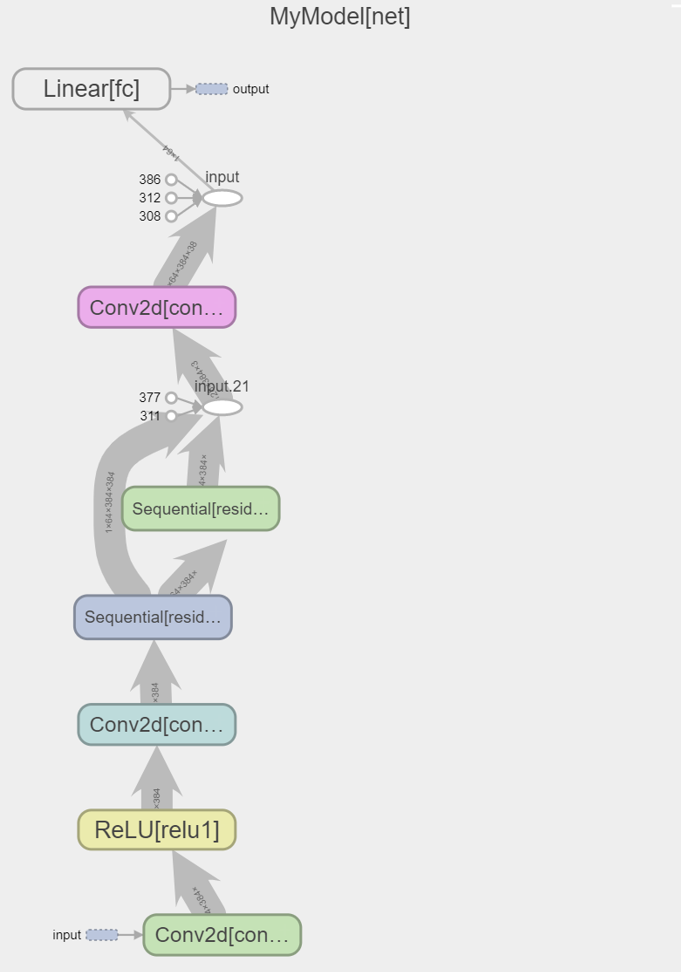
\includegraphics[width=0.3\textwidth]{figures/MyModel.png}
	\caption{Schemat Blokowy Sieci MyModel}
	\label{fig:dane1}
  \end{figure}

\clearpage
\section{Przedstwienie oraz omówienie archtektury sieci  tf mobilenetv3 small minimal 100 }


Sieć tf\_mobilenetv3\_small\_minimal\_100 to zredukowana wersja modelu MobileNetV3 w implementacji dla TensorFlow. Jest to model o architekturze sieci konwolucyjnej z milionem parametrów do uczenia, który został zoptymalizowany pod kątem wydajności i ma mniejszą liczbę parametrów niż pełna wersja MobileNetV3.

Główne cechy sieci tf\_mobilenetv3\_small\_minimal\_100 to:

\begin{itemize}

\item Warstwy konwolucyjne: Sieć wykorzystuje zestaw warstw konwolucyjnych o różnych rozmiarach jądra (3x3, 5x5 itp.) w celu ekstrakcji cech z obrazu wejściowego. Warstwy konwolucyjne są stosowane sekwencyjnie, tworząc głębsze reprezentacje obrazu.

\item Bloki Bottleneck: Wykorzystuje bloki Bottleneck, które składają się z sekwencji warstw konwolucyjnych o mniejszej liczbie filtrów, aby zmniejszyć liczbę parametrów. Te bloki pomagają zachować wydajność i dokładność modelu przy ograniczonych zasobach obliczeniowych.

\item Ekspresywność: Model ma na celu osiągnięcie wysokiej ekspresywności przy niskiej złożoności. Wykorzystuje różne techniki, takie jak konwolucje separowalne, tzw. "squeeze-and-excite" (SE) oraz aktywacje "hard-swish", aby zwiększyć reprezentatywność modelu.

\item Minimalne rozmiary: Sieć tf\_mobilenetv3\_small\_minimal\_100 ma mniejszą liczbę parametrów niż pełna wersja MobileNetV3, co sprawia, że jest bardziej odpowiednia do zastosowań o ograniczonych zasobach obliczeniowych, takich jak urządzenia mobilne.

\item Celem tej sieci jest dostarczenie efektywnego modelu o mniejszej liczbie parametrów, który może być wykorzystywany w zasobooszczędnych środowiskach, jednocześnie zachowując odpowiednią dokładność w zadaniach klasyfikacji obrazów.
\end{itemize}

\begin{figure}[ht]
	\centering
	\begin{subfigure}[b]{0.4\textwidth}
	  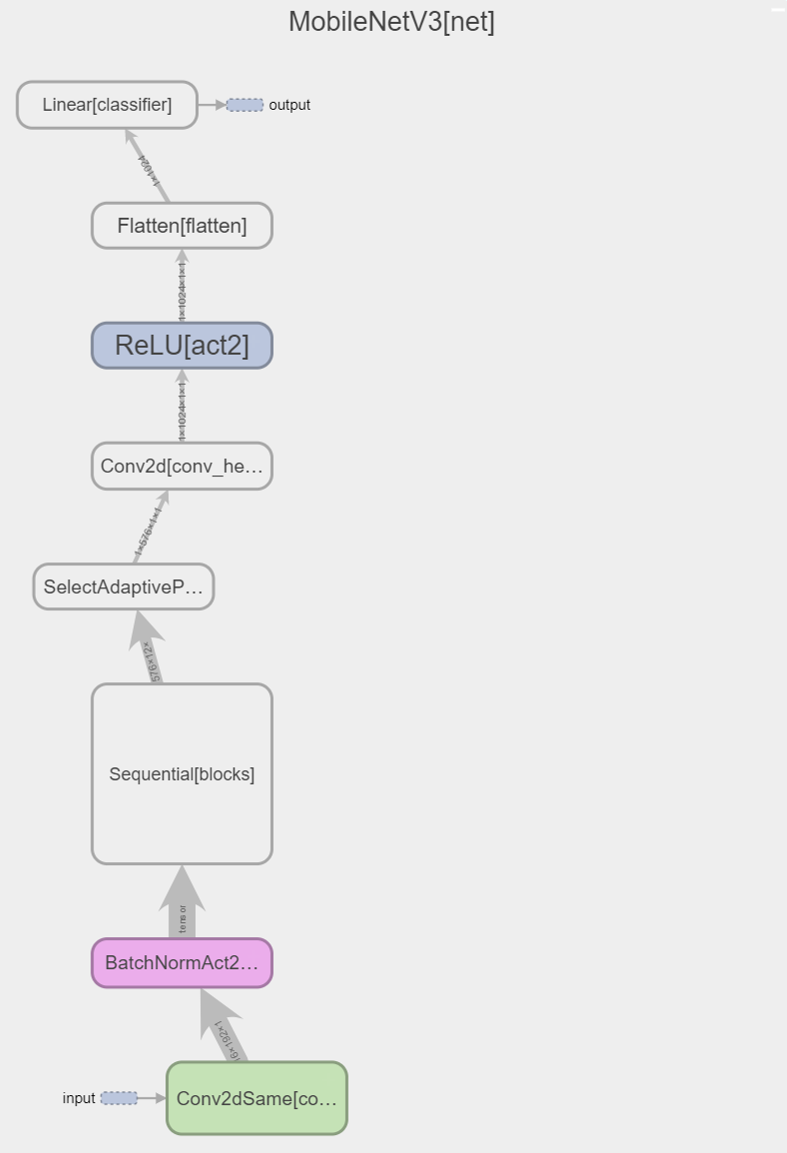
\includegraphics[width=\textwidth]{figures/v3_main.png}
	  \caption{Główne bloki struktury sieci}
	  \label{fig:obraz1}
	\end{subfigure}
	\hfill
	\begin{subfigure}[b]{0.4\textwidth}
	  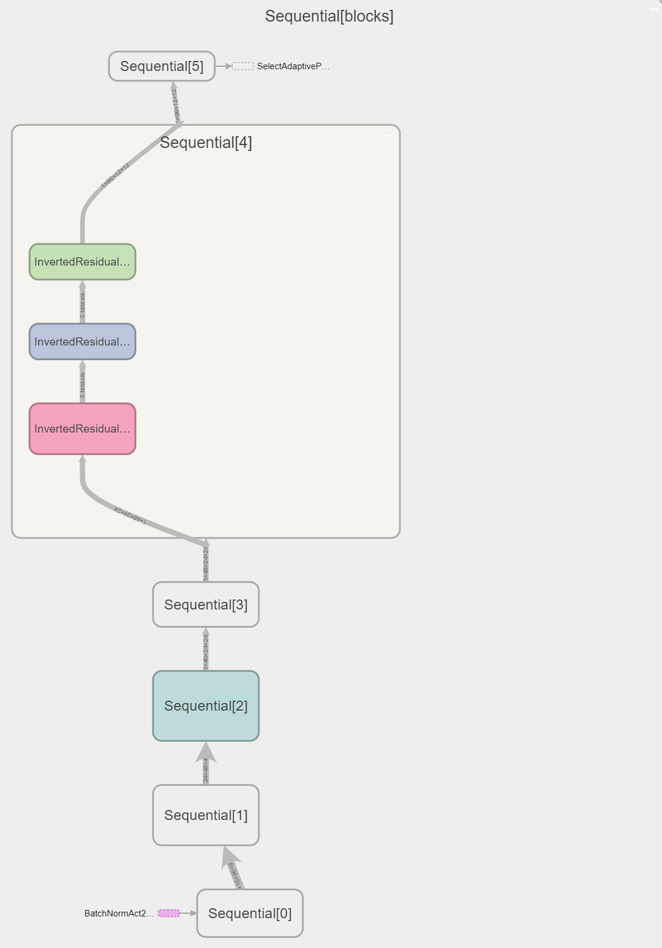
\includegraphics[width=\textwidth]{figures/v3_seq.png}
	  \caption{Rosrzeżony blok Sequential  }
	  \label{fig:obraz2}
	\end{subfigure}
	\caption{Struktura sieci tf\_mobilenetv3\_small\_minimal\_100}
	
\end{figure}

\clearpage

\section{Omówienie klasy LightningModule oraz optymalizatora ADAM}
Klasa LightningModule służy między innymi do rejsteracji Hiperparametrów sieci, obróbki danych wejściowych, oraz procesu uczenia się sieci.

Optymalizator Adam łączy w sobie zalety dwóch innych algorytmów optymalizacji: AdaGrad, który dostosowuje krok uczenia dla każdego parametru na podstawie historycznych gradientów, i RMSProp, który stosuje średnią ruchomą gradientu.

Kluczowe aspekty działania optymalizatora Adam są następujące:
\begin{itemize}
	
\item Średnia ruchoma gradientu (first moment): Algorytm Adam przechowuje średnią ruchomą gradientu, która jest obliczana na podstawie historycznych gradientów. Ta średnia ruchoma reprezentuje estymację momentu pierwszego (optymalizacja kierunku).

\item Kwadrat średniej ruchomej gradientu (second moment): Algorytm Adam przechowuje średnią ruchomą kwadratu gradientu, która jest obliczana na podstawie historycznych kwadratów gradientów. Ta średnia ruchoma reprezentuje estymację momentu drugiego (optymalizacja kroku).

\item Bias korekcyjny: Ze względu na inicjalne przesunięcie obliczeń średnich ruchomych, Adam stosuje bias korekcyjny w celu uwzględnienia tego efektu i poprawienia stabilności w początkowych iteracjach optymalizacji.

\item Aktualizacja parametrów: Algorytm Adam aktualizuje parametry sieci na podstawie estymacji momentu pierwszego i momentu drugiego. Wykorzystuje również dodatkowy hiperparametr, tzw. współczynnik uczenia (learning rate), który kontroluje wielkość kroku aktualizacji.

\item Działanie optymalizatora Adam może być podsumowane w kilku krokach: obliczanie gradientu dla aktualnych parametrów, obliczanie estymacji momentu pierwszego i momentu drugiego, uwzględnianie biasu korekcyjnego, obliczanie nowych wartości parametrów na podstawie estymacji momentów i współczynnika uczenia.

\end{itemize}

\begin{figure}[h]
	\centering
	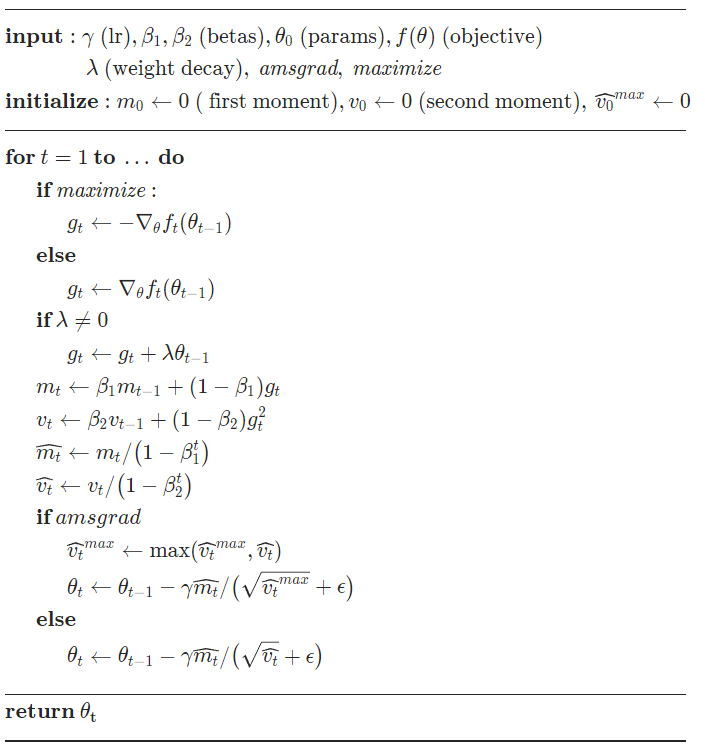
\includegraphics[width=0.7\textwidth]{figures/ADAM.png}
	\caption{Matematyczny zapis Optymalizatora ADAM}
	\label{fig:312}
\end{figure}


\section{Eksperyment I. badanie parametru rozmiaru wsadu oraz wielkości zdjęcia }


Rozmiar wsadu (batch size) jest parametrem określającym liczbę próbek, które są przetwarzane jednocześnie podczas jednej iteracji algorytmu uczenia maszynowego. Zmiana rozmiaru wsadu może mieć wpływ na proces uczenia się z kilku powodów:

 \begin{itemize}
	\item Wydajność obliczeniowa: Większy rozmiar wsadu może przyspieszyć proces uczenia, ponieważ możliwe jest równoległe przetwarzanie większej liczby próbek na jednostce obliczeniowej. Dzieje się tak, ponieważ przetwarzanie wsadów odbywa się z wykorzystaniem efektywnych operacji macierzowych, które mogą być zoptymalizowane na poziomie sprzętowym.

\item Stabilność uczenia: Przy mniejszych rozmiarach wsadu, gradienty obliczane na podstawie próbek są bardziej losowe i bardziej zmienne, co może prowadzić do większej niestabilności procesu uczenia. Większy rozmiar wsadu może przyczynić się do bardziej stabilnego uczenia poprzez wygładzenie gradientów i zmniejszenie wpływu pojedynczych próbek na aktualizację wag.

\item Zużycie pamięci: Większy rozmiar wsadu wymaga większej ilości pamięci do przechowywania danych i gradientów. Jeśli dostępna pamięć jest ograniczona, konieczne może być dostosowanie rozmiaru wsadu tak, aby zmieścił się w dostępnej pamięci.

\item Ogólna dokładność modelu: Wybór rozmiaru wsadu może mieć wpływ na ogólną dokładność modelu. Przy większych rozmiarach wsadu model może mieć lepszą zdolność uogólniania, ponieważ jest trenowany na większej liczbie różnorodnych przykładów. Jednak mniejszy rozmiar wsadu może prowadzić do bardziej szczegółowych aktualizacji wag, które mogą doprowadzić do osiągnięcia lepszej lokalnej dokładności.

 \end{itemize}

 Wielkość zdjęcia ma istotny wpływ na proces uczenia się w modelach opartych na sieciach neuronowych. Oto kilka aspektów, które należy wziąć pod uwagę:

\begin{itemize}
	\item Ilość dostępnej informacji: Większe zdjęcia zawierają więcej pikseli, co oznacza większą ilość informacji. Model może zyskać dostęp do bardziej szczegółowych cech obrazu, co może przyczynić się do lepszej wydajności w zadaniach takich jak rozpoznawanie obiektów czy segmentacja.
 
 \item Złożoność obliczeniowa: Przetwarzanie większych obrazów wymaga większej mocy obliczeniowej. Modele uczące się na większych obrazach mogą być bardziej wymagające obliczeniowo i potrzebować większych zasobów, takich jak pamięć GPU i czas treningu.
 

 \item Overfitting: Jeśli model jest zbyt skomplikowany lub ma zbyt mało dostępnych danych treningowych w porównaniu do wielkości obrazów, istnieje ryzyko przeuczenia (overfittingu). Model może nauczyć się "zapamiętywać" konkretne obrazy treningowe zamiast generalizować cechy. W takich przypadkach można rozważyć zastosowanie technik regularyzacji, takich jak augmentacja danych lub wczytywanie obrazów w mniejszych rozmiarach.
 
 \item Efektywność obliczeniowa: Przetwarzanie większych obrazów może być bardziej czasochłonne, zarówno podczas treningu, jak i podczas wykonywania predykcji na nowych danych. Dla niektórych zastosowań, takich jak detekcja obiektów w czasie rzeczywistym, może być konieczne dostosowanie rozmiaru zdjęcia do wymagań czasowych.
 

\end{itemize}


\subsection{Metoda badawcza}

Celem tego eksperymentu jest znalezienie optymalnych parametrów dla sieci neuronowych poprzez zmianę rozmiaru partii (batch size) oraz rozmiaru obrazu. Przeprowadzony zostanie szereg testów, gdzie batch size będzie przyjmował wartości: 2, 4, 8, 16, 32, 64, 128, 256, a rozmiar obrazu będzie wynosił: 10, 65, 121, 177, 232, 288, 344, 400.

W trakcie każdego testu, oba modele (netV3 i MyModel) zostaną wytrenowane przy użyciu odpowiednich wartości batch size i rozmiaru obrazu. Następnie, dokładność (accuracy) oraz funkcja straty (loss) zostaną zmierzone i zarejestrowane .
\begin{lstlisting}[language=Python,caption=Kod do ekperymentu II, label={kod_Transformacja}]
  lr=1e-4
  max_epochs=10
  for batch_size in vec_batch_size:
    for img_size in vec_img_size:

      model = ClasyficatorCNN(slect_model_timm = select_model  , size = img_size ,batch_size=batch_size ,lr=lr, pretrained=pretrained)
      logger = TensorBoardLogger("lightning_logs", name=select_model+ "img_size = " + str(img_size)+ "batch_size = "+str(batch_size), default_hp_metric=False)
      trainer = Trainer(
          max_epochs=max_epochs,
          logger=logger)
      trainer.fit(model)
      
      vec_loss = np.append(vec_loss  , model.loss)
      vec_acc  = np.append(vec_acc  , model.valid_acc)
      vec_pres = np.append(vec_pres , model.val_precision)
      vec_acu  = np.append(vec_acu , model.val_ACU)
      vac_sens = np.append(vac_sens , model.val_specificitys)


      model = ClasyficatorCNN(slect_model = MyModel()  , size = img_size ,batch_size = batch_size,lr=lr, pretrained=pretrained)
      logger = TensorBoardLogger("lightning_logs", name=select_model+ "img_size = " +  str(img_size)+"batch_size = "+str(batch_size) , default_hp_metric=False)
      trainer = Trainer(
          max_epochs=max_epochs,
          logger=logger)
      trainer.fit(model)
      vec_loss_Mymodel = np.append(vec_loss  , model.loss)
      vec_acc_Mymodel  = np.append(vec_acc  , model.valid_acc)
      vec_pres_Mymodel  = np.append(vec_pres , model.val_precision)
      vec_acu_Mymodel  = np.append(vec_acu , model.val_ACU)
      vac_sens_Mymodel  = np.append(vac_sens , model.val_specificitys)
\end{lstlisting}

\subsection{Wyniki}
Nie udało się przeprowadzić całego testu został on przerwany na wielkość wsadu = 8. Przerwanie to uniemożliwia optymalne dobranie parametrów, jednak można zauważyć kilka interesujących zjawisk. Na przykład, mały rozmiar wsadu wpływa na szybkie przeuczenie modelu, niezależnie od rozmiaru zdjęcia.

Ponadto, można zauważyć różnicę w liczbie potrzebnych iteracji do przejścia przez jedną epokę w zależności od wartości batch size. Przy tej samej liczbie epok, ilość iteracji rośnie odwrotnie proporcjonalnie do rozmiaru wsadu.
\begin{figure}[h]
	\centering
	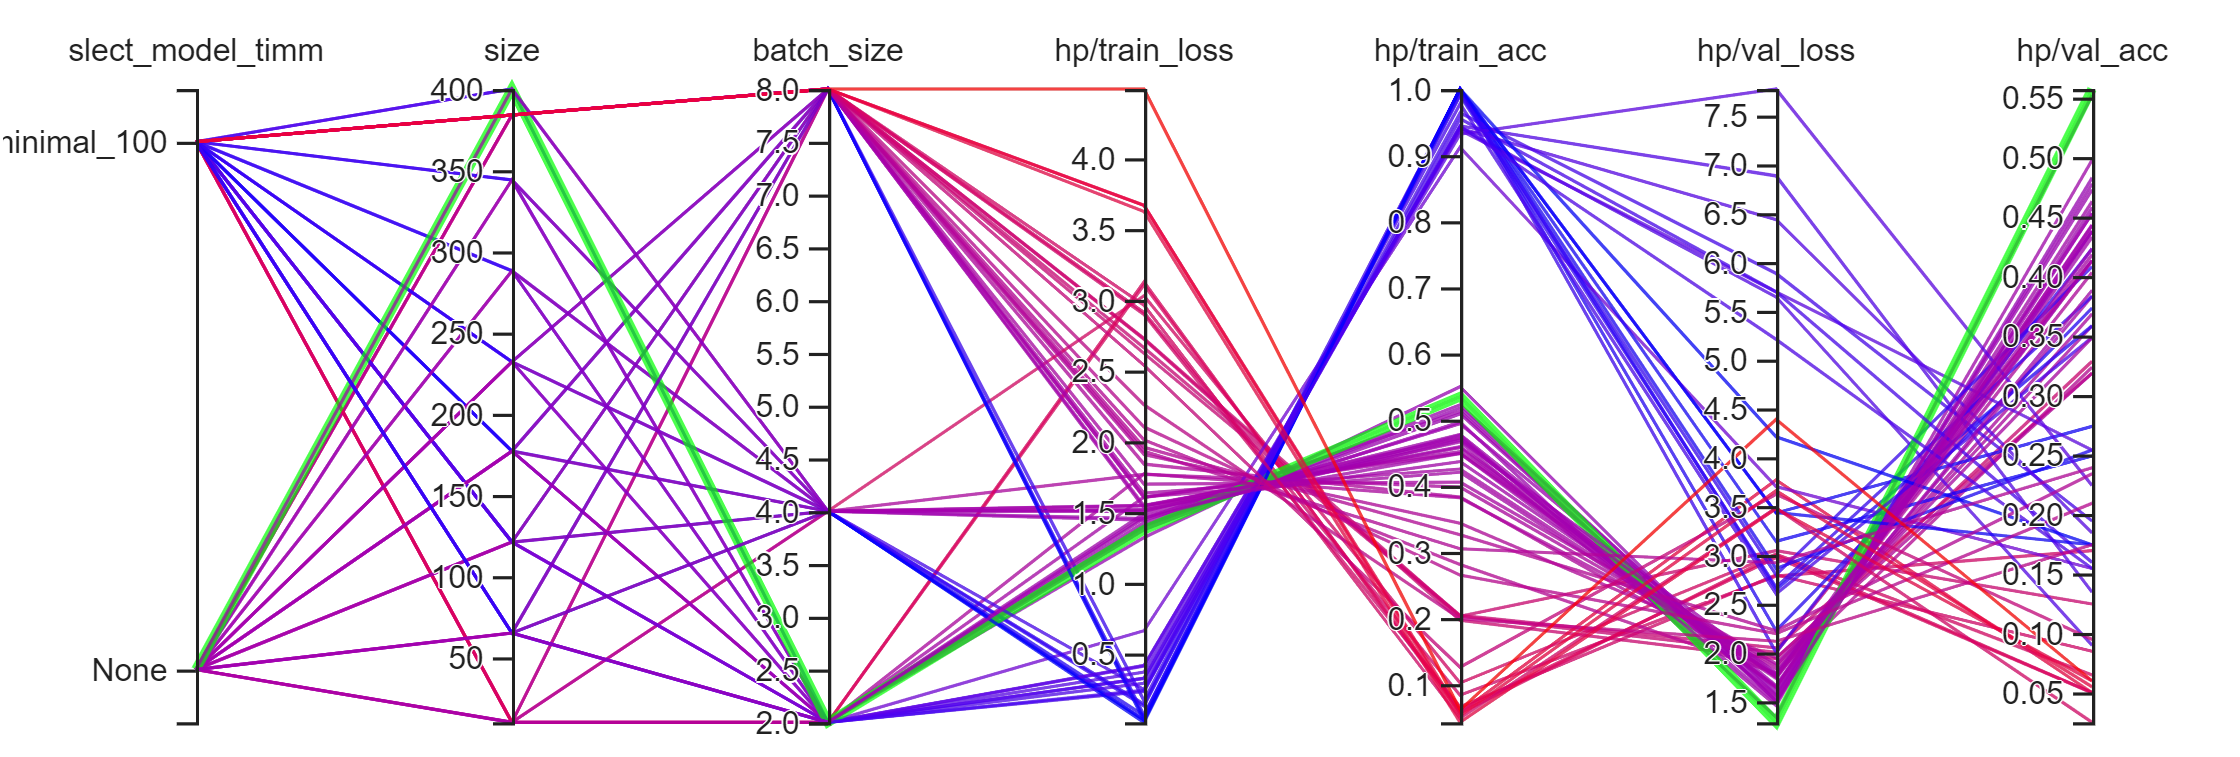
\includegraphics[width=1\textwidth]{figures/myModelbest.png}
	\caption{Najlepsze zbadane rozwiązaqnie dla MyModel1}
	\label{fig:123432}
\end{figure}
\begin{figure}[h]
	\centering
	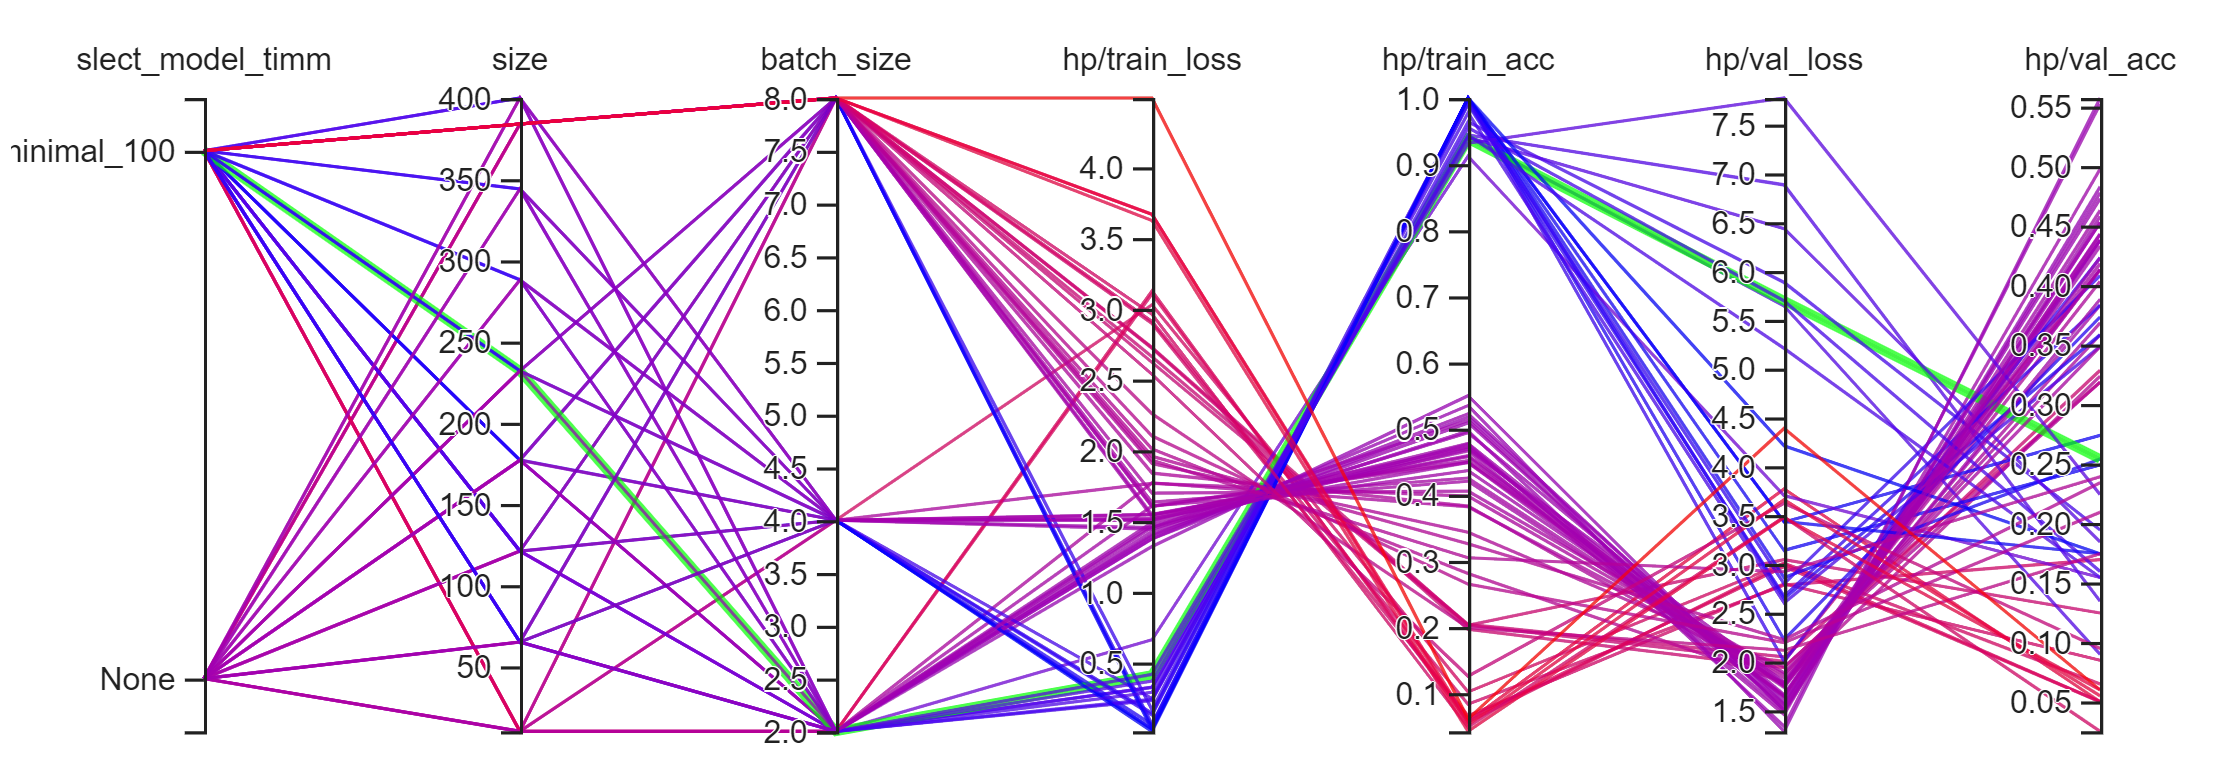
\includegraphics[width=1\textwidth]{figures/netv3best.png}
	\caption{Njalepsze możliwe rozwiązanie dla NetV3}
	\label{fig:da2352ne}
\end{figure}


\begin{figure}[ht]
	\centering
	\begin{subfigure}[b]{0.4\textwidth}
	  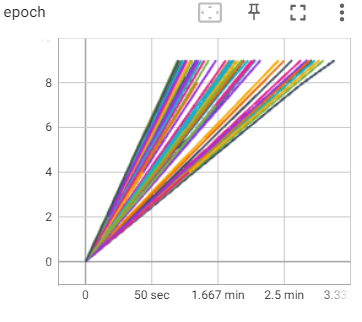
\includegraphics[width=\textwidth]{figures/epokiodczasu.png}
	  \caption{stosunek czasu do epok }
	  \label{fig:obraz1}
	\end{subfigure}
	\hfill
	\begin{subfigure}[b]{0.4\textwidth}
	  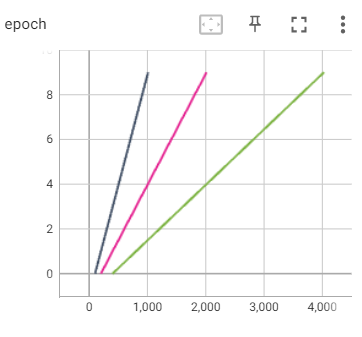
\includegraphics[width=\textwidth]{figures/epokiodilościkroków.png}
	  \caption{stosunek ilości epok do iteracji }
	  \label{fig:obraz2}
	\end{subfigure}
	\caption{Zestawienie szybkości nauczania }
	
\end{figure}
\begin{figure}[ht]
	\centering
	\begin{subfigure}[b]{0.4\textwidth}
	  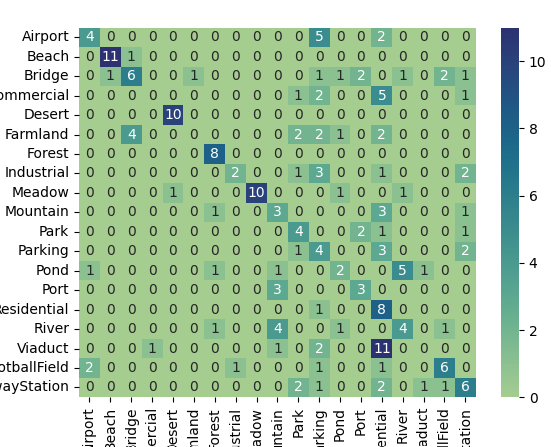
\includegraphics[width=\textwidth]{figures/cmdlav3.png}
	  \caption{Macierz pomyłek dla NetV3}
	  \label{fig:obraz1}
	\end{subfigure}
	\hfill
	\begin{subfigure}[b]{0.4\textwidth}
	  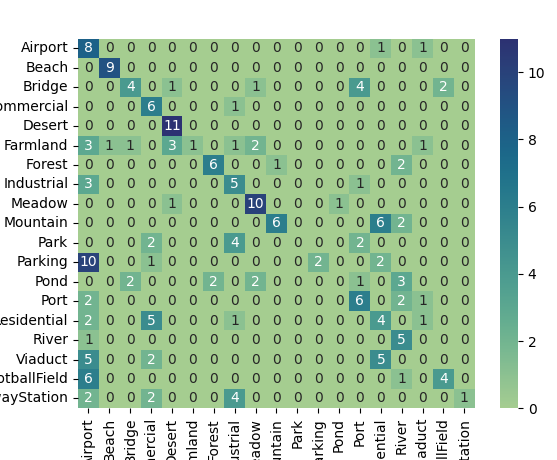
\includegraphics[width=\textwidth]{figures/cdmdlaMymodel.png}
	  \caption{Macierz pomyłek dla MyModel1}
	  \label{fig:obraz2}
	\end{subfigure}
	\caption{zstwawienie macierzy pomyłek}
	
\end{figure}

\clearpage
\section{Eksperyment II. Uczenie i porównanie modeli po 200 epokach}

W celu porównania skuteczności modeli MyModel i NetV3, przeprowadzimy eksperyment polegający na uczeniu obu modeli przez 200 epok. Porównamy wyniki dla modelu MyModel oraz modelu NetV3

\subsection{Metoda badawcza}
Na podstawie wyników z porzedniego zostały dobrane paramety sieci dla architektury Mymodel1 batch\_size $=$ 8 img\_size $=$ 400, dla archtektury tf\_mobilenetv3\_small\_minimal\_100 batch\_size $=$ 2 img\_size $=$ 232. Po przeprowadzenia procesu uczenia  Listing \ref{uczenia}
zostanie przepowadzona anaaliza wyników szybkości (ilości iteracji podczas uczenia) oraz taki hiper parametrów jak dokładność, czułość , precyzja, oraz pole pod krrzywą ROC
\begin{lstlisting}[language=Python,caption=Kod do ekperymentu II. ,label={uczenia}]
    lr = 3e-4
    batch_size = 2
    model = ClasyficatorCNN(slect_model= MyModel1(), size = 400 ,batch_size=8 ,lr=lr)
    logger = TensorBoardLogger("lightning_logs", name="My model  bbatch_size:" , default_hp_metric=True)
    trainer = Trainer(
        max_epochs=200,
        logger=logger
    )
    trainer.fit(model)

    select_model = 'tf_mobilenetv3_small_minimal_100'
    model = ClasyficatorCNN(slect_model_timm = select_model  , size = 232 ,batch_size=2,lr=lr,pretrained=False)
    logger = TensorBoardLogger("lightning_logs", name=select_model, default_hp_metric=False)
    trainer = Trainer(
        max_epochs=200,
        logger=logger
    )
    trainer.fit(model)

    model = ClasyficatorCNN(slect_model_timm = Kod do ekperymentu II , size = 232 ,batch_size=2,lr=lr,pretrained=True)
    logger = TensorBoardLogger("lightning_logs", name=select_model, default_hp_metric=False)
    trainer = Trainer(
        max_epochs=200,
        logger=logger
    )
    trainer.fit(model)
\end{lstlisting}

\subsection{Wyniki}


Podczas procesu uczenia zastosowano trzy modele sieci oparte na architekturze tf\_mobilenetv3\_small\_minimal\_100. Analiza wyników pokazała, że tylko dwa z tych modeli osiągnęły dokładność na poziomie bliskim 0.8, natomiast trzeci model był dotknięty efektem przeuczenia.

Okazało się, że modele oparte na architekturze tf\_mobilenetv3\_small\_minimal\_100 nie były w stanie wykorzystać w pełni swojego potencjału, co można przypisać złemu doborowi parametrów lub zbyt małemu zbiorowi uczącemu. W przypadku modelu version\_0, nieprzetrenowanego, nie był w stanie uogólniać cech, skupiając się zbyt mocno na dopasowaniu do danych uczących. Wskazuje na to porównanie funkcji błędów dla danych uczących i testowych. Aby rozwiązać ten problem, można by rozważyć zwiększenie rozmiaru zbioru uczącego.

Drugi model, version\_1, oparty na architekturze tf\_mobilenetv3\_small\_minimal\_100, okazał się przetrenowany, co oznacza, że był w stanie bardzo szybko osiągnąć wysoką dokładność na danych uczących. Niemniej jednak, istnieje ryzyko, że taki model może mieć trudności z ogólną zdolnością do uogólniania na nowe dane spoza zbioru uczącego.

Trzeci model, oparty na własnej architekturze MyModel1, również osiągnął dobre wyniki podczas procesu uczenia, ale jego tempo nauki było znacznie wolniejsze. Mimo to, model ten zdolny był efektywnie uczyć się i osiągnąć wysoką dokładność.




\begin{figure}[h]
	\centering
	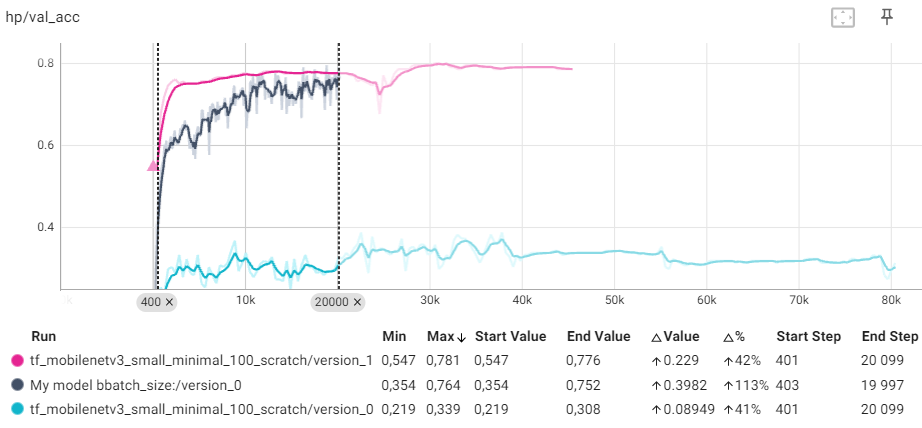
\includegraphics[width=0.9\textwidth]{figures/hp_val_acc.png}
	\caption{Zestawienie dokładnośći poszczególnych modeli}
	\label{fig:dreg2ne}
\end{figure}

\begin{figure}[ht]
	\centering
	\begin{subfigure}[b]{0.9\textwidth}
	  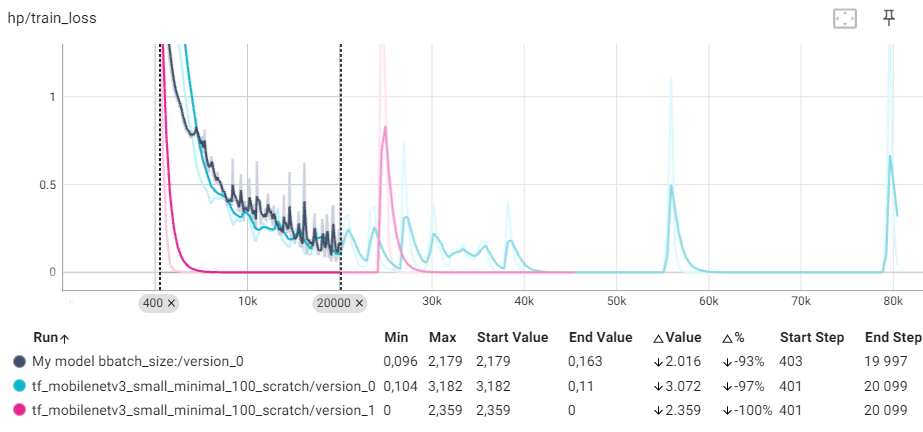
\includegraphics[width=\textwidth]{figures/hp_train_loss.png}
	  \label{fig:obraz1}
	\end{subfigure}
	\hfill
	\begin{subfigure}[b]{0.9\textwidth}
	  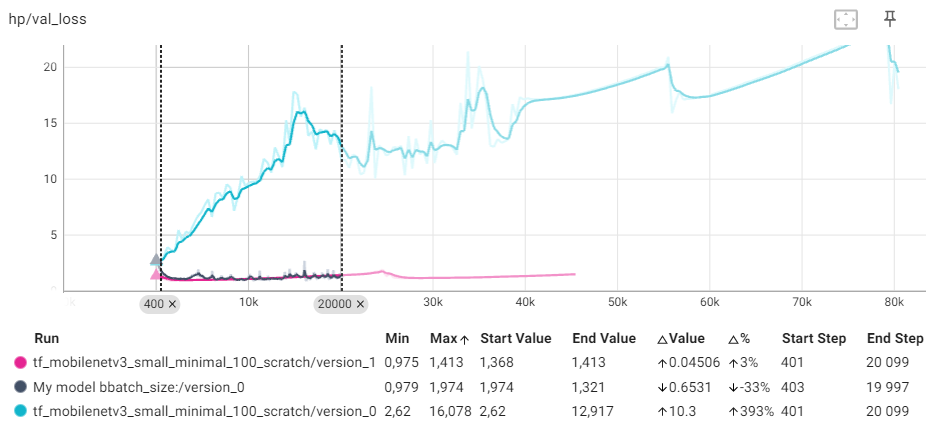
\includegraphics[width=\textwidth]{figures/hp_val_loss.png}
	  \label{fig:obraz2}
	\end{subfigure}
	\caption{Porównie wykesów błędów dla danych validacyjnych oraz trenigowych}
	
\end{figure}

\begin{figure}[h]
	\centering
	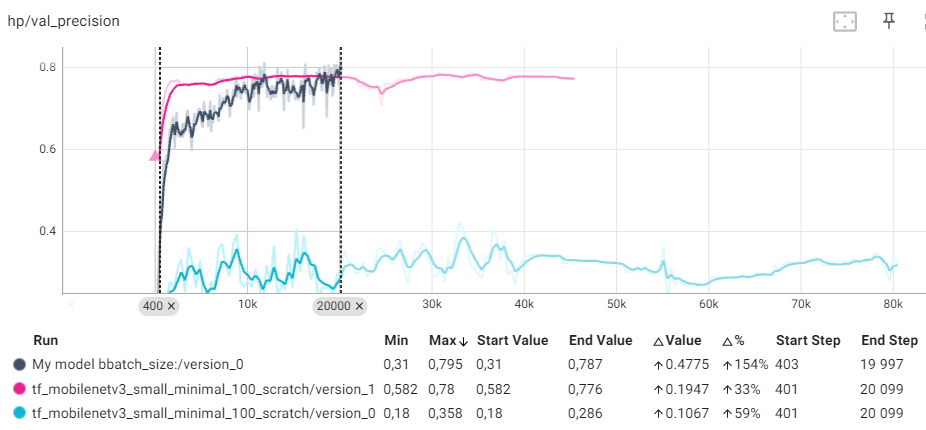
\includegraphics[width=0.9\textwidth]{figures/hp_val_pre.png}
	\caption{Zestawienie precyzji poszczególnych modeli}
	\label{fig:wsef52ne}
\end{figure}

\begin{figure}[h]
	\centering
	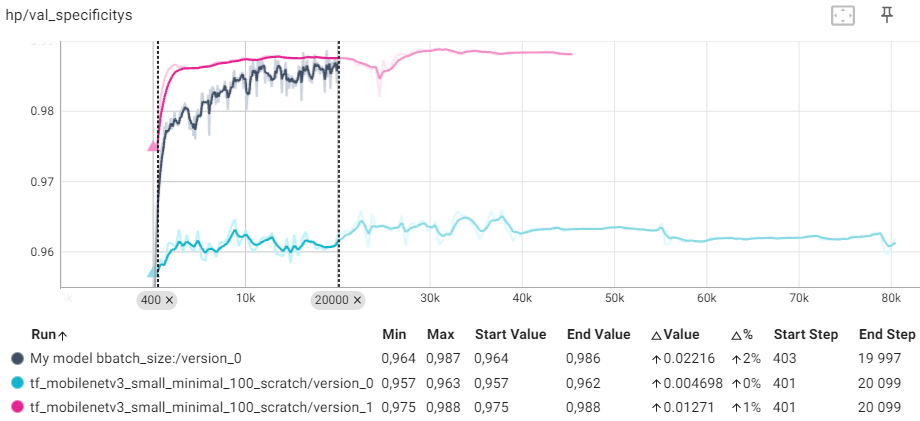
\includegraphics[width=0.9\textwidth]{figures/hp_val_spec.png}
	\caption{Zestawienie czułości poszczególnych modeli}
	\label{fig:dasfe352ne}
\end{figure}

\begin{figure}[h]
	\centering
	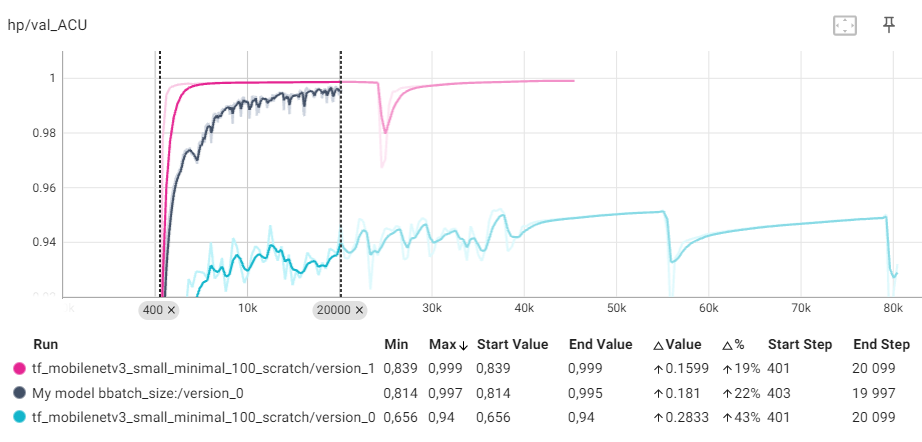
\includegraphics[width=0.9\textwidth]{figures/hp_valACU.png}
	\caption{Zestaweinie wartości pola pod krzywą ROC poszczególnych modeli}
	\label{fig:dareg352ne}
\end{figure}



\begin{figure}[ht]
	\centering
	\begin{subfigure}[b]{0.45\textwidth}
	  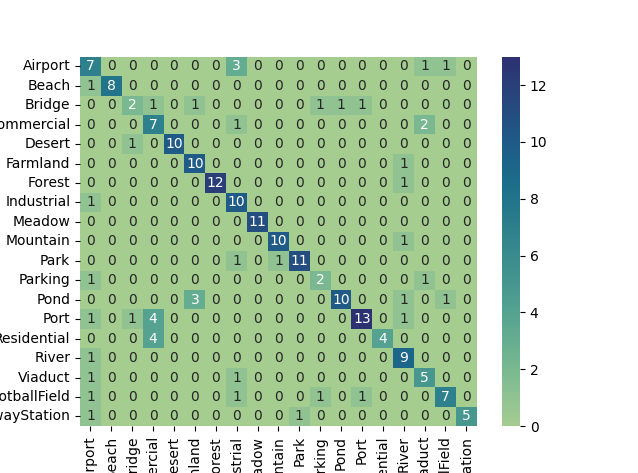
\includegraphics[width=\textwidth]{figures/cmv3_exp2.png}
	  \label{fig:obraz1}
	\end{subfigure}
	\hfill
	\begin{subfigure}[b]{0.45\textwidth}
	  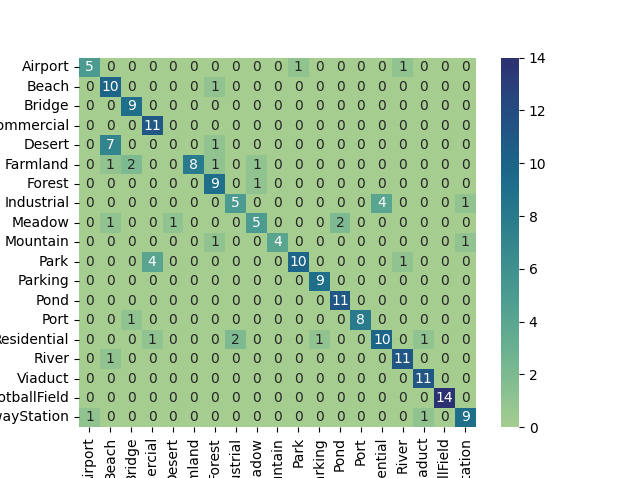
\includegraphics[width=\textwidth]{figures/cmMM_exp2.png}
	 
	  \label{fig:obraz2}
	\end{subfigure}
	\caption{zstwawienie macierzy pomyłek}
	
\end{figure}


\begin{figure}[ht]
	\centering
	\begin{subfigure}[b]{0.45\textwidth}
	  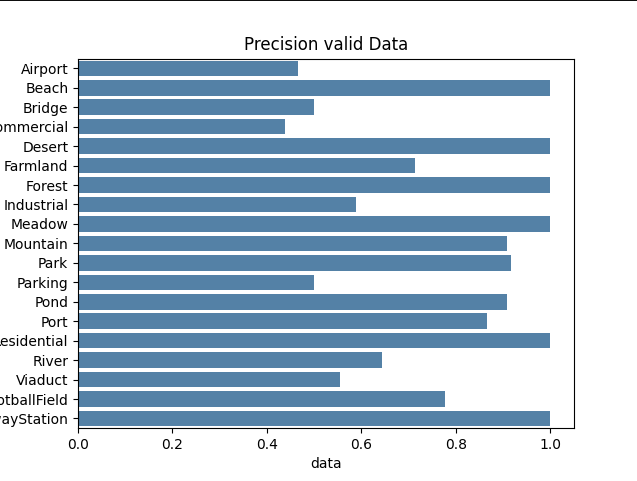
\includegraphics[width=\textwidth]{figures/barv3_exp2.png}
	  \label{fig:obraz1}
	\end{subfigure}
	\hfill
	\begin{subfigure}[b]{0.45\textwidth}
	  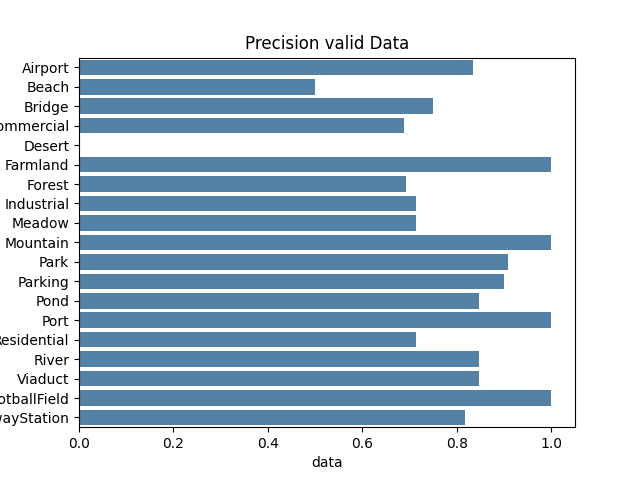
\includegraphics[width=\textwidth]{figures/barMM_exp2.png}
	  \label{fig:obraz2}
	\end{subfigure}
	\caption{zstwawienie wykresów precyzj dla poszczególnych klas}
	
\end{figure}



\clearpage

\section{Podsumowanie}

Niniejsza praca miała na celu zgłębienie problematyki i rozważenie różnych rozwiązań związanych z głębokimi sieciami konwolucyjnymi (CNN) w kontekście klasyfikacji obrazów. W toku badań skupiono się na problemie zanikającego gradientu, który często utrudnia efektywne uczenie się w głębokich sieciach. Przedstawiono i omówiono różnorodne techniki mające na celu przeciwdziałanie temu zjawisku, takie jak stosowanie funkcji aktywacji ReLU, inicjalizacja wag przy użyciu metody Xavier/Glorot, normalizacja danych lub warstw oraz wykorzystanie architektur sieci z połączeniami pomijającymi.

Funkcja aktywacji ReLU okazała się popularnym wyborem w głębokich sieciach neuronowych, ze względu na jej zdolność do skutecznego rozwiązywania problemu zanikającego gradientu. Metoda inicjalizacji wag za pomocą Xavier/Glorot umożliwia odpowiednie skalowanie wag na początku procesu uczenia, zapobiegając tym samym zanikaniu gradientu. Wykorzystanie normalizacji danych lub warstw przyczynia się do zmniejszenia zakresu wartości wejściowych i ułatwia proces uczenia. Architektury sieci z połączeniami pomijającymi umożliwiają przekazywanie informacji o niskopoziomowych cechach, co sprzyja skutecznemu uczeniu sieci.

W ramach pracy zaprezentowano również dwie konkretne architektury sieci: własną architekturę CNN oraz architekturę sieci tf mobilenetv3 small minimal 100. Szczegółowo omówiono kluczowe cechy tych struktur i ich zastosowanie w kontekście klasyfikacji obrazów.

Przeprowadzono również dwa eksperymenty, których celem było zbadanie wpływu różnych parametrów na skuteczność uczenia sieci. Pierwszy eksperyment koncentrował się na badaniu rozmiaru wsadu oraz rozmiaru zdjęć, podczas gdy drugi eksperyment porównywał modele po 200 epokach uczenia. Wyniki eksperymentów dostarczyły istotnych informacji na temat optymalnych parametrów oraz skuteczności uczenia sieci.

W pracy omówiono również klasę LightningModule oraz optymalizator ADAM, które zostały wykorzystane w procesie uczenia sieci.

Do przeprowadzenia badań wykorzystano zbiór danych WHU-RS19, który zawierał różne klasy obiektów na zdjęciach. Przeprowadzono odpowiednie przetwarzanie danych, takie jak zmiana rozmiaru zdjęć i konwersja ich do formatu tensorów, aby umożliwić efektywne uczenie sieci.

W trakcie przeprowadzanych eksperymentów zastosowano dwa modele: netV3 oraz MyModel. Każdy z modeli był trenowany przy użyciu określonych wartości batch size i rozmiaru obrazu. Celem eksperymentów było zmierzenie dokładności (accuracy) oraz funkcji straty (loss) i zbadanie wpływu różnych czynników na proces uczenia.

Niestety, nie udało się przeprowadzić pełnego testu, ponieważ został on przerwany przy batch size równym 8. Przerwanie eksperymentu uniemożliwiło optymalne dobranie parametrów, jednakże obserwowane zjawiska są nadal interesujące. Na przykład, mały rozmiar batch size prowadził do szybkiego przeuczenia modelu, niezależnie od rozmiaru zdjęcia.

Dodatkowo, zaobserwowano różnicę w liczbie iteracji potrzebnych do przejścia przez jedną epokę w zależności od wartości batch size. Przy tej samej liczbie epok, ilość iteracji wzrastała odwrotnie proporcjonalnie do rozmiaru batch size.

W przypadku trzeciego modelu, opartego na własnej architekturze MyModel1, osiągnięto dobre wyniki podczas procesu uczenia, ale tempo nauki było znacznie wolniejsze. Mimo to, model ten był zdolny do skutecznego uczenia się i osiągnięcia wysokiej dokładności.


\clearpage
\addcontentsline{toc}{section}{Literatura}


\begin{thebibliography}{4}
\bibitem{str} https://pytorch.org/docs/stable/index.html. Dostęp 29.05.2023.
\bibitem{str2} https://lightning.ai/docs/pytorch/stable/. Dostęp 29.05.2023.
\bibitem{str3} https://lightning.ai/docs/pytorch/latest/. Dostęp 29.05.2023.
\bibitem{wyk} Kluska j.: Prezentacja z cyklu wykładów S.I. pt. Classifiers assessment methods
,Rzeszow University of Technology.

\end{thebibliography}





\end{document}


Głębokie sieci neuronowe stanowią potężne narzędzie w dziedzinie klasyfikacji obrazów, ale napotykają na pewne wyzwania. Zanikający gradient jest jednym z głównych problemów, który utrudnia skuteczne uczenie się sieci. Aby temu zaradzić, można stosować techniki, takie jak funkcja aktywacji ReLU, inicjalizacja wag z wykorzystaniem metody Xavier/Glorot oraz normalizacja danych lub warstw.

Funkcja aktywacji ReLU jest popularna ze względu na swoją prostotę i zdolność do rozwiązania problemu zanikającego gradientu. Inicjalizacja wag metodą Xavier/Glorot pozwala na równomierne rozprowadzenie wariancji i uniknięcie problemów z gradientem na początku uczenia. Normalizacja danych lub warstw przyczynia się do stabilnego procesu optymalizacji poprzez zmniejszenie zakresu wartości wejściowych. Dodatkowo, architektury sieci z połączeniami pomijającymi umożliwiają przekazywanie informacji o niskopoziomowych cechach bezpośrednio do warstw wyższego poziomu, co przyczynia się do lepszej klasyfikacji i predykcji